%!TEX root = ../main.tex
While we considered using various features for the character recognition such as crossing, projection histograms and celled projections \cite{HWR:features1}\cite{HWR:features2}. From all the above the celled projections report the best results (7\% and 10\% better than crossings and projections respectively) \cite{HWR:features1}.

Celled projections are extracted as follows. First the area of the character is split into regions, vertically, horizontally or mixed. In \ref{fig:method:features:feature} we see an example of vertical projection. Then for each of the regions we acquire the projections of the pixels on the left border of the region. This way binary vectors are created which then we concatenate.

\begin{figure}[ht]
	\label{fig:method:features:feature}
	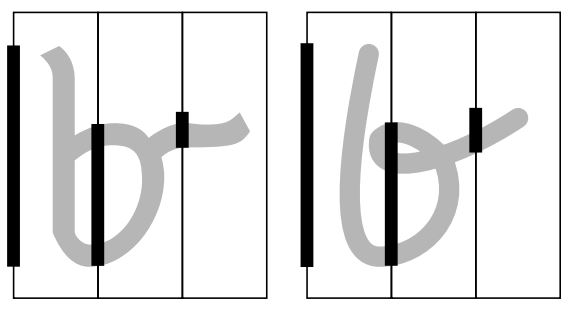
\includegraphics[width=8cm]{shared/img/projection_letter.jpg}
	\caption{In the above picture we see that even if the characters are differently written the projection feature will still extract consistent vectors.}
\end{figure}